\documentclass{article}

% NeurIPS 2025 style, final copy (no line numbers)
\PassOptionsToPackage{numbers,square,sort,compress}{natbib}
\usepackage[main, final]{neurips_2025}

\usepackage[utf8]{inputenc}
\usepackage[T1]{fontenc}
\usepackage{hyperref}
\usepackage{url}
\usepackage{booktabs}
\usepackage{amsfonts}
\usepackage{amsmath}
\usepackage{nicefrac}
\usepackage{microtype}
\usepackage{graphicx}
\usepackage{xcolor}
\setcitestyle{numbers,square,comma,compress,sort}

\title{Sensor-Light Closed-Loop Ultrafiltration Control in Haemodialysis:\\ An In-Silico Feasibility Study on Routine Machine Data}

\author{%
  LE YI \\
  Matriculation number: G2605168D \\
  MSc in Artificial Intelligence in Medicine \\
  Lee Kong Chian School of Medicine, Nanyang Technological University \\
  \texttt{MD6329 Deep Learning for Healthcare AI} \\
}

\begin{document}
\makeatletter
\renewcommand{\@noticestring}{Course project report, MD6329 Deep Learning for Healthcare AI, NTU LKCMedicine, 2026.}
\makeatother
\maketitle

\begin{abstract}
Intradialytic hypotension (IDH) is among the most frequent complications of haemodialysis. Clinical
closed-loop systems that adjust the ultrafiltration rate (UFR) already exist, but they rely on optical
relative-blood-volume sensors that a wearable device cannot easily carry. This project asks whether
routinely recorded dialysis-machine data alone can support a predict-then-adjust loop, and what such a
loop would cost. Using HEMOBP (CC~BY~4.0; 1{,}072 patients recorded, 919 remaining after cleaning,
160{,}069 analysable sessions), we predict IDH in the remainder of a session from information available
at a decision point $T$, with patient-level splits and AUPRC as the primary metric. Five models are
compared. At the 60-minute decision point the best model reaches AUPRC 0.2015 against a 0.0586 prevalence baseline, but
patient-level bootstrap intervals are wide (95\% CI 0.13--0.28) and the gap to the compact 1D-CNN+MLP
is not established (difference 0.018, 95\% CI $-0.001$ to 0.033), so we do not rank architectures. Raw
probabilities are unusable as risks: they over-predict by a factor of four to six and every Brier score
is worse than the no-skill value, which Platt scaling on validation repairs (0.052 versus 0.055).
In the XGBoost ablation, pre-decision blood pressure carried the largest share of predictive information (removing it
costs 44\% of AUPRC) while machine-setting features added little independent value under the evaluated feature set. An exploratory action-conditioned
simulation, with candidates generated only from the pump setting observed at $T$, illustrates the
trade-off rather than validating a policy: holding that setting implies 7.3\% predicted risk with
131~mL residual, while a model-chosen reduction gives 5.9\% with 354~mL --- paired patient-level bootstraps put that
difference at 1.4 points (95\% CI 1.1--1.7), but the same model both chose and scored the action, only 65\% of candidates
have conditional support, and the risk model is conditional rather than identified. The control section is
therefore reported as a sensitivity analysis; establishing an intervention effect requires
prospective data.

\end{abstract}

\section{Problem Formulation}

Haemodialysis replaces kidney function intermittently. Between sessions, patients accumulate fluid; during a four-hour session a machine must remove that fluid at a rate the cardiovascular system can tolerate. When the ultrafiltration rate (UFR) exceeds the capillary refill rate, effective circulating volume falls and intradialytic hypotension (IDH) follows. In our cohort, 11.2\% of sessions reach a nadir systolic blood pressure (SBP) below 90~mmHg.

Three generations of countermeasures exist. First, reactive control: a proportional--integral--derivative (PID) controller, or nursing judgement, reacts only after blood pressure has already fallen. Second, blood-volume biofeedback: commercial systems such as Hemocontrol (Baxter) and the BVM/BTM-based feedback of Fresenius adjust UFR and dialysate conductivity in closed loop, guided by an optical sensor that measures relative blood volume \citep{santoro1998biofeedback,ronco2000biofeedback,dong2024closedloop}. Third, machine-learning prediction, which forecasts IDH from clinical variables but has rarely been evaluated as a component of a control loop \citep{bi2022lstm,idhmstf2025}.

For the second generation, some studies report benefit while a recent review concludes that evidence for clinical adoption
is still under evaluation \citep{dong2024closedloop}. It also depends on an optical relative-blood-volume sensor; on the
basis of the design project's own component assumptions that sensor is bulky and costly relative to a wearable envelope, but
we did not verify those specifications here, so we treat this as a design motivation rather than an established fact. This motivates the question we study here: \emph{with routinely recorded machine data only --- pump settings, dialysate parameters, and the sparse blood-pressure readings nurses already take --- can a predict-then-adjust loop be built, and what does it cost?}

We decompose this into three testable sub-questions, each mapped to a claim from an accompanying engineering design project: (i) how early and how accurately can IDH be predicted (claim C1/C2); (ii) is multi-modal sensing necessary, and which modality matters (C3); (iii) what predicted-risk, fluid-removal and session-time trade-offs appear under exploratory action-conditioned simulations
(C4/C5) --- with a fourth question about whether observational data can support causal claims at all (C6).

The work is deliberately positioned against the course material: irregular EHR time series (Lecture~5, \textasciitilde 00:38), recurrent models (Lecture~6, \textasciitilde 02:14), the Transformer (Lecture~7, \textasciitilde 00:27 and \textasciitilde 27:16), multi-modal fusion (Lecture~8, \textasciitilde 00:11), the reinforcement-learning view of sequential decisions (Lecture~10, \textasciitilde 00:27), interpretability (Lecture~11, \textasciitilde 05:11) and privacy in federated deployments (Lecture~12, \textasciitilde 00:39) \citep{md6329lectures}. Software 3.0 (generative AI) was used early here, to survey the closed-loop ultrafiltration literature and to test whether the design project's "prediction beats PID" framing was defensible. It was not (Section~2), and correcting that framing changed the research question rather than its wording.

\section{Related Work}

\paragraph{Closed-loop ultrafiltration.} Santoro et al. introduced a multivariable closed-loop controller that adjusts UFR and dialysate conductivity to follow a target blood-volume trajectory, cutting severe hypotensive episodes from 26 to 3 in a crossover study \citep{santoro1998biofeedback}. Ronco et al. found fewer hypotensive episodes and better equilibrated Kt/V under biofeedback \citep{ronco2000biofeedback}. A recent narrative review located 28 clinical studies, of which 23 reported effectiveness and none reported adverse effects, while concluding that evidence for clinical adoption still requires randomised trials \citep{dong2024closedloop}. Our work does not compete with these systems; it asks what can be done when their sensor is unavailable.

\paragraph{IDH definitions and epidemiology.} Prevalence depends heavily on definition \citep{kuipers2019prevalence}, and different definitions carry different mortality associations \citep{flythe2015idh}. Guidelines recommend keeping the ultrafiltration rate below roughly 13~mL/kg/h, alongside ultrafiltration profiling and cooler dialysate \citep{kdoqi2005cvd,china2022consensus}. We therefore report three definitions and justify the one we adopt.

\paragraph{Machine learning for IDH.} Tree ensembles and recurrent networks dominate the recent literature; a bidirectional LSTM reached 78.5\% accuracy and AUC 0.822 on 73{,}323 sessions \citep{bi2022lstm}, and a multi-scale temporal feature model reported 98.1\% AUC with XGBoost on a public cohort \citep{idhmstf2025}. A Temporal Fusion Transformer reached AUC 0.953 but at high compute cost. Two gaps motivate our design: prediction is rarely coupled to a control evaluation, and the causal status of the ultrafiltration signal is rarely examined. We address both, and we quantify the fluid-removal price of acting on a prediction. Our modelling choices also follow the course treatment of irregular clinical time series, recurrent gating, and attention over short sequences \citep{md6329lectures}.

\section{Data}

\paragraph{Cohort.} HEMOBP \citep{lin2019hemobp} contains dialysis-machine recordings linked to hospital demographic data, released under CC~BY~4.0: 1{,}072 patients, 4{,}366{,}298 intra-session readings. Sessions are not a calendar day --- the unit runs three shifts and the last crosses midnight --- so we reconstruct sessions as contiguous runs of readings separated by more than six hours, and assign each to a dialysis day beginning at 08:00. The source cohort thus contains 1{,}072 patients and 197{,}269 reconstructed sessions. Eligibility filtering
(Table~\ref{tab:flow}) leaves 160{,}069 sessions from \textbf{919 patients} before the horizon-specific exclusions, and it is
those 919 patients that every modelling result describes --- not the 1{,}072 recorded. The start-weight filter is the single
largest loss and is what removes 153 of them.

\begin{table}[t]
\caption{Sample flow. Rows 1--5 are the session-level cleaning steps (each row is the number of sessions remaining
after that filter); the lower block is the horizon-specific exclusion that turns eligible sessions into modelling samples (\texttt{no readings} = 8 sessions present in the weight file but absent from the
machine-reading file).}
\label{tab:flow}
\centering
\begin{tabular}{lrrrr}
\toprule
& T=30 & T=60 & T=90 & T=120 \\
\midrule
sessions reconstructed & 197{,}269 & 197{,}269 & 197{,}269 & 197{,}269 \\
$-$ duration outside 60--480 min & 196{,}457 & 196{,}457 & 196{,}457 & 196{,}457 \\
$-$ start weight outside 20--200 kg & 162{,}563 & 162{,}563 & 162{,}563 & 162{,}563 \\
$-$ interdialytic gain outside $-2$ to 10 kg & 160{,}673 & 160{,}673 & 160{,}673 & 160{,}673 \\
$-$ mean UFR outside 0--20 mL/kg/h & 160{,}069 & 160{,}069 & 160{,}069 & 160{,}069 \\
\midrule
eligible sessions & 160{,}069 & 160{,}069 & 160{,}069 & 160{,}069 \\
$-$ session shorter than $T$+30~min & 0 & 244 & 567 & 1{,}160 \\
$-$ fewer than 3 pre-$T$ readings & 12{,}798 & 8{,}468 & 3{,}192 & 1{,}071 \\
$-$ no post-$T$ readings & 30 & 45 & 83 & 155 \\
$-$ already below 90~mmHg before $T$ & 3{,}658 & 4{,}260 & 5{,}458 & 6{,}493 \\
$-$ no machine readings & 8 & 8 & 8 & 8 \\
\midrule
modelling samples & 143{,}575 & 147{,}044 & 150{,}761 & 151{,}182 \\
\bottomrule
\end{tabular}
\end{table}

\paragraph{Descriptive statistics.} Mean session duration is 236 $\pm$ 24.5 minutes; mean UFR is 8.26 $\pm$ 3.38~mL/kg/h (median 7.8), i.e.\ mostly below the guideline threshold of 13; median interdialytic weight gain is 2.32~kg. Crucially, blood pressure is sparse: the median within-session interval between distinct readings is 50.7 minutes, and only 32\% of intervals are at or below 20 minutes (Figure~\ref{fig:eda}).

\begin{figure}[t]
\centering
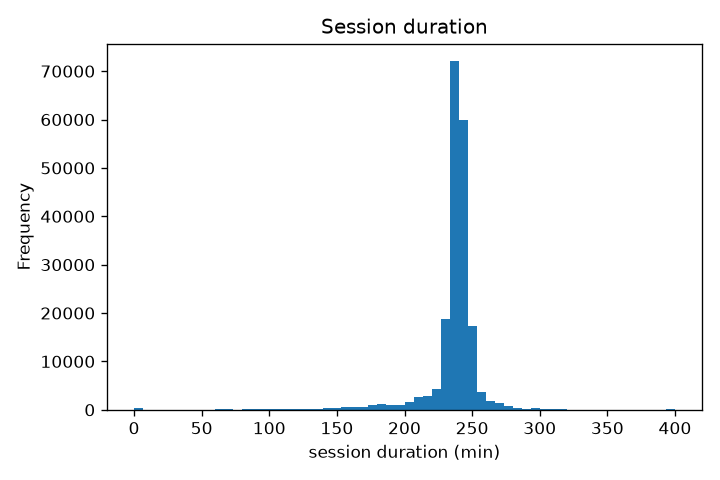
\includegraphics[width=0.49\linewidth]{figs/fig_duration.png}
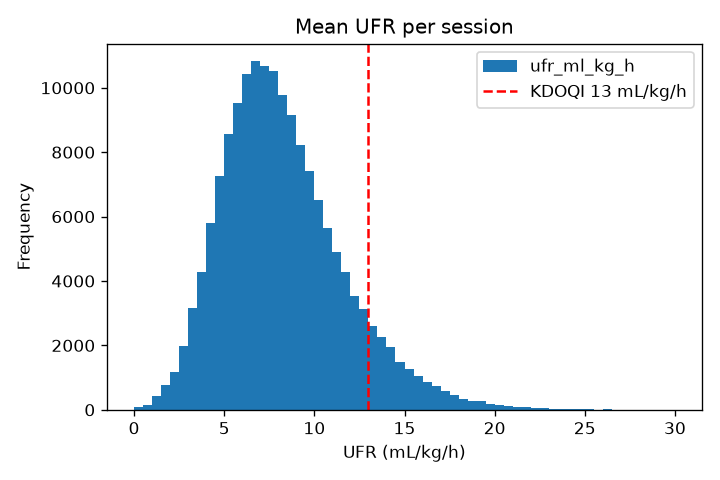
\includegraphics[width=0.49\linewidth]{figs/fig_ufr.png}
\caption{Cohort descriptives. Left: session duration. Right: mean UFR per session against the 13~mL/kg/h guideline threshold.}
\label{fig:eda}
\end{figure}

\paragraph{Outcome definition.} Table~\ref{tab:idh} reports three candidate definitions. A drop of $\ge$20~mmHg applies to 84.4\% of sessions and is therefore unusable as a target; we adopt nadir SBP $<$90~mmHg (11.24\%) as primary and report nadir $<$100~mmHg (20.73\%) for sensitivity.

\begin{table}[t]
\caption{IDH incidence under three definitions (session level, $n$=197{,}269).}
\label{tab:idh}
\centering
\begin{tabular}{lcc}
\toprule
Definition & Incidence & Use \\
\midrule
nadir SBP $<$ 90~mmHg & 11.24\% & primary \\
nadir SBP $<$ 100~mmHg & 20.73\% & sensitivity \\
max $-$ nadir $\ge$ 20~mmHg & 84.42\% & rejected (non-specific) \\
\bottomrule
\end{tabular}
\end{table}

\paragraph{Sampling design.} For each session we form one sample per decision point $T \in \{30,60,90,120\}$ minutes. Inputs use only readings with time $\le T$; the label is the nadir SBP of readings after $T$. Sessions already below 90~mmHg before $T$ are excluded, since the prediction would be moot; sessions with fewer than three pre-$T$ readings are excluded. This yields 143{,}575 (T=30), 147{,}044 (T=60), 150{,}761 (T=90) and 151{,}182 (T=120) samples, with remaining-window IDH rates of 8.0\%, 7.7\%, 7.1\% and 6.5\% respectively. As a qualitative example, take one test session at $T$=60~min: 1.88~L of interdialytic gain, 0.46~L already removed, 1.42~L still to remove, 2.42~h remaining, and a clinician-chosen 0.48~L/h for the remainder. That plan removes 1.16~L and therefore leaves 266~mL unremoved, while SBP drifts from 148 to a nadir of 110~mmHg and no IDH event occurs. Sessions like this are where the label becomes noisy at the margin, and they are also where the fluid trade-off in E5 bites. Cleaning follows pre-registered bounds (duration 60--480~min, weight 20--200~kg, interdialytic gain $-2$ to 10~kg, UFR 0--20~mL/kg/h): 197{,}269 sessions reduce to 160{,}069 eligible.

\paragraph{Limitations of the data.} HEMOBP is \emph{in-centre} haemodialysis: four hours, supine, with sparse cuff measurements. It contains no photoplethysmography, electrocardiography, inertial or relative-blood-volume signals, and no symptom or nursing-intervention records. It therefore cannot validate a five-to-fifteen-minute warning window, and it cannot represent the ambulatory wearable scenario described in the accompanying design project. We return to this mismatch in the discussion.

\section{Approach}

\paragraph{Framing.} The primary task is classification: given the state at $T$, will this session reach a nadir SBP below 90~mmHg afterwards? Trajectory prediction appears only \emph{inside} the control simulation (Section~\ref{sec:e5}), where a dynamics model must answer ``what if the remaining ultrafiltration profile were different?'' Reporting classification as the main result keeps the headline numbers interpretable and avoids over-claiming.

\paragraph{Features and modalities.} Fifteen features fall into three groups, which we later ablate: (a) \emph{demographic/static} --- age, sex, diabetes, start weight, dry weight, interdialytic weight gain; (b) \emph{pre-$T$ physiology} --- first SBP, nadir so far, SBP slope, count of distinct readings; (c) \emph{machine settings} --- mean UFR, blood flow, dialysate conductivity and temperature up to $T$. Sequence models additionally consume up to 96 readings of seven channels (SBP, DBP, UFR, blood flow, conductivity, dialysate temperature, normalised elapsed time) with an explicit padding mask.

\paragraph{Models.} Five models are compared. (1) XGBoost \citep{chen2016xgboost} on tabular features is the clinical baseline. (2) A multilayer perceptron consumes static features only. (3) A 1D-CNN+MLP fusion mirrors the architecture of the accompanying design project: a convolutional branch over the reading sequence, an MLP branch over static features, concatenated before a shared head. (4) An LSTM \citep{hochreiter1997lstm} reads the masked sequence and takes the last valid hidden state. (5) A Transformer encoder built from scratch reuses the encoder written for the course assignment on clinical sequences \citep{md6329assignment}: sinusoidal positional encoding, multi-head scaled dot-product attention with key-padding masks, GELU feed-forward blocks and mean pooling over valid positions \citep{vaswani2017attention}.

\paragraph{Evaluation protocol.} Splits are by patient (70/15/15) with a fixed seed, because a patient contributes dozens of sessions and row-wise splitting would leak. AUPRC is the primary metric given class imbalance; AUROC, Brier score and sensitivity at 80\% specificity are secondary. Because AUPRC is prevalence-sensitive, we report test prevalence alongside every value.

\paragraph{Training procedure.} All four neural models share one training recipe, which reduces tuning-related variation; the models nevertheless consume
different inputs (static features only for the MLP, sequence plus static features for the fusion model, sequence-dominant
inputs for the LSTM and the Transformer), so E1 compares complete modelling pipelines rather than isolating architecture
alone. Inputs are standardised with training-split statistics only: each sequence channel is centred and scaled over valid (non-pad) training entries and re-zeroed at padded positions, and the fifteen static features are standardised with training-split mean and standard deviation. Training minimises binary cross-entropy with \texttt{pos\_weight} set to the training-split negative-to-positive ratio (17.1:1 at $T$=60); optimisation is Adam with learning rate $10^{-3}$ and batch size 256, for at most ten epochs, with early stopping of patience two epochs on validation AUPRC and restoration of the best-validation checkpoint before test evaluation. Dropout is 0.2 in the fusion and head layers and 0.1 inside the Transformer encoder, which uses $d$=64, four heads and two layers. Python, NumPy and PyTorch seeds are all fixed to 42. XGBoost uses the histogram tree method, 600 trees of depth 6, learning rate 0.05, 0.8 row and column subsampling, and \texttt{scale\_pos\_weight} equal to the same ratio. These defaults are revisited in E7.

\paragraph{Control policies (in silico).}\label{sec:e5}
The control analysis rests on an \emph{action-conditioned risk model}, not on an identified counterfactual model. It adds two
features to the tabular set --- a planned remaining UFR and the remaining minutes --- and is fitted on pairs of (state at $T$,
the UFR clinicians actually went on to deliver). It therefore estimates $P(\text{IDH}\mid\text{state},\text{plan})$ on the
distribution of plans clinicians chose; it does not identify what would happen under a plan that was rarely or never chosen.
Arms are generated only from what a controller knows at $T$: the \emph{pump setting observed at $T$} (the last non-zero
setting at or before $T$) is the anchor, and candidates are $\{1.0,0.9,0.8,0.7,0.6\}\times$ that setting. Each candidate is
then entered into the model as the planned remaining UFR, which is a simplification: it assumes the plan would be held,
whereas a real device would react continuously. The arms are
\emph{hold} (keep the setting), \emph{reactive} (cut 30\% if SBP has fallen $\ge$15~mmHg or nadir is below 100), and
\emph{predictive} (minimise predicted risk subject to a residual-fluid tolerance). The trajectory clinicians followed is
reported only as a descriptive reference, because it was not a choice available at $T$. All quoted risks are Platt-recalibrated
with parameters fitted on the validation split. This section is a sensitivity analysis of the trade-off; it is not a
validation of a control policy.

\paragraph{Causal plausibility diagnostics.} Two probes examine the internal consistency of the ultrafiltration signal and
its exposure to confounding; they do not identify a causal effect. First, a perturbation sweep: we vary the planned remaining UFR multiplier from 0.3 to 1.3 and record mean predicted risk, plus the crude observed association between actual UFR and IDH. Second, an intervention-style ablation on the Transformer: zeroing the attention output or the feed-forward output of each encoder block (the intervention tooling follows \citealp{wu2024pyvene}) and measuring the change on the logit scale (not the probability scale, which saturates). Figure~\ref{fig:e6} shows the perturbation and association results.

\paragraph{Software 3.0.} Generative AI assistance was used throughout, under the course honour code, and is disclosed here. It was most valuable in three places: refactoring the session builder after pandas-groupby iteration failed on 160k sessions (a vectorised rewrite cut runtime from $>$20~min to 19~min for four horizons); diagnosing a misleading ablation result in an earlier assignment that turned out to be sigmoid saturation rather than a modelling failure; and localising a device-placement bug in a diagnostic model. It was least reliable on domain judgement --- choosing the IDH definition, deciding what the control comparison may legitimately claim, and recognising that the biofeedback literature makes ``predictive versus PID'' the wrong framing. All numerical results in this report were produced by scripts in the accompanying repository and can be regenerated.

\section{Experiments}

\paragraph{E1: five-model comparison.} Table~\ref{tab:e1} reports the 60-minute decision point on 22{,}407 test samples (the label covers the remainder of the
session, not the following 60 minutes)
(prevalence 5.86\%). The from-scratch Transformer has the highest point estimate, but patient-level bootstrap intervals are
wide and overlap: it exceeds the 1D-CNN+MLP by 0.018 with a 95\% interval of $-0.001$ to 0.033
(Figure~\ref{fig:e9ci}). We therefore \emph{do not} claim an architecture ranking; what the comparison supports is that a
compact fused model is competitive at a quarter of the parameters. Two cautions follow. The validation AUPRC values used for checkpoint selection (up to 0.32) sit above the test values reported here; validation
carries 24{,}665 samples at 6.29\% prevalence against 22{,}407 at 5.86\% on test, so a prevalence difference accounts for
part of the gap, and selecting the best of ten checkpoints on validation accounts for another part. We report both numbers
rather than attribute the gap to a single cause. And every Brier score exceeds the no-skill value
$p(1-p)=0.0552$, so they cannot be read as calibration quality; E8 diagnoses why and repairs it.

\begin{table}[t]
\caption{E1: five models at $T$=60~min (test $n$=22{,}407, prevalence 5.86\%). Intervals are patient-level bootstrap
($B$=1{,}000). Brier scores are raw and all exceed the no-skill 0.0552 (E8).}
\label{tab:e1}
\centering
\begin{tabular}{lcccccc}
\toprule
Model & AUPRC & 95\% CI & AUROC & Sens@80\%spec & Brier & Params \\
\midrule
XGBoost & 0.1675 & 0.118--0.221 & 0.733 & 0.548 & 0.116 & --- \\
MLP & 0.1721 & 0.107--0.257 & 0.758 & 0.562 & 0.150 & 10{,}369 \\
\textbf{1D-CNN+MLP} & 0.1837 & 0.117--0.268 & 0.768 & 0.573 & 0.136 & 24{,}961 \\
LSTM & 0.1804 & 0.119--0.247 & 0.761 & 0.569 & 0.175 & 32{,}129 \\
Transformer & 0.2015 & 0.131--0.282 & 0.774 & 0.587 & 0.164 & 107{,}265 \\
\bottomrule
\end{tabular}
\end{table}


\begin{figure}[t]
\centering
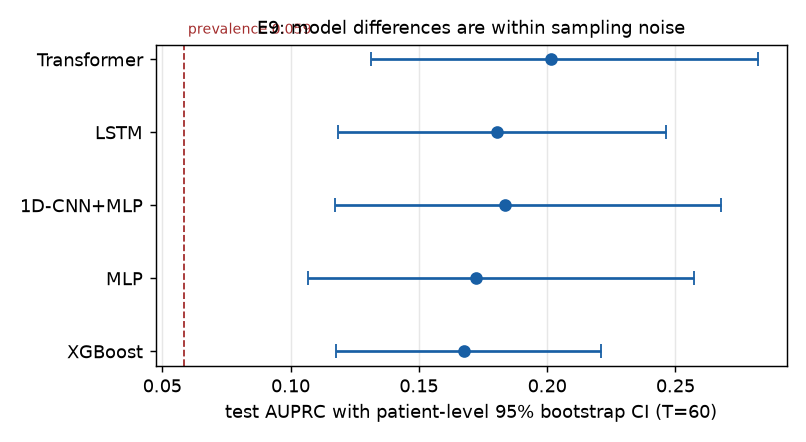
\includegraphics[width=0.55\linewidth]{figs/fig_e9_ci.png}
\caption{E9: test AUPRC with patient-level 95\% bootstrap intervals. The intervals overlap across all five models, so the
architecture ordering in Table~\ref{tab:e1} is not established.}
\label{fig:e9ci}
\end{figure}
\begin{figure}[t]
\centering
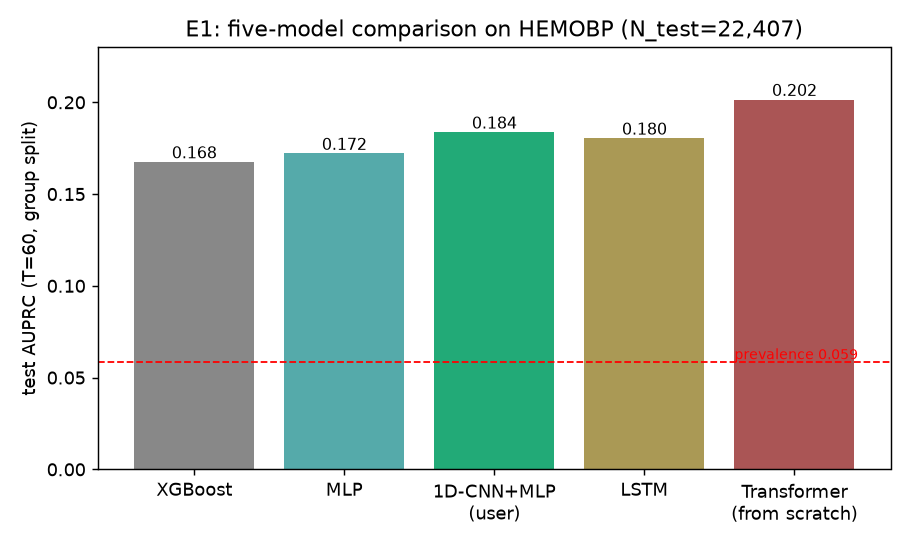
\includegraphics[width=0.62\linewidth]{figs/fig_e1_models.png}
\caption{E1: AUPRC by model against the no-skill prevalence line.}
\label{fig:e1}
\end{figure}

\paragraph{E2: compute budget.} Table~\ref{tab:e2} shows why the fusion model is the reasonable deployment choice: 0.271~ms per sample on CPU and 3.31~ms for a batch of 256, against 1.487~ms and 147.2~ms for the Transformer --- 44$\times$ faster at batch scale, while remaining competitive under the default comparison settings (E1/E9). Latency was measured on a laptop (RTX~3070~Ti, CPU fallback) and is indicative, not an embedded-MCU benchmark. LSTM FLOPs are under-counted by the profiler because recurrent terms are not attributed; we do not compare on that column.

\begin{table}[t]
\caption{E2: accuracy versus cost ($T$=60). Latency on CPU; FLOPs per sample.}
\label{tab:e2}
\centering
\begin{tabular}{lcccc}
\toprule
Model & Params & FLOPs & Lat.\ bs1 & Lat.\ bs256 \\
\midrule
XGBoost & 600 trees & --- & 0.003~ms & --- \\
1D-CNN+MLP & 24{,}961 & 1.22~M & 0.271~ms & 3.31~ms \\
LSTM & 32{,}129 & 0.06~M$^*$ & 0.544~ms & 9.85~ms \\
Transformer & 107{,}265 & 23.69~M & 1.487~ms & 147.2~ms \\
\bottomrule
\end{tabular}
\end{table}

\paragraph{E3: prediction horizon.} Table~\ref{tab:e3} shows a non-monotone pattern: quality peaks at $T$=90~min for the fusion model (AUPRC 0.2395, AUROC 0.807). Two effects trade off --- later decision points have more observed history, but their remaining windows contain fewer events, so prevalence falls from 6.21\% to 4.75\%. Cross-$T$ comparisons therefore mix window and prevalence effects and must not be read as ``later is better''. The practically important point is the floor: with blood pressure sampled every 50.7 minutes at the median, prediction horizons below roughly one sampling interval cannot be validated on this data. The five-to-fifteen-minute warning requirement specified in the accompanying design project therefore cannot be validated
at this sampling frequency. Continuous physiological sensing, including photoplethysmography, remains a hypothesis for future
investigation; its incremental predictive value would have to be established on data that actually contain such signals.

\begin{table}[t]
\caption{E3: horizon study. 1D-CNN+MLP AUPRC/AUROC by decision point.}
\label{tab:e3}
\centering
\begin{tabular}{lcccc}
\toprule
$T$ (min) & 30 & 60 & 90 & 120 \\
\midrule
Test prevalence & 6.21\% & 5.86\% & 5.20\% & 4.75\% \\
XGBoost AUPRC & --- & 0.1675 & 0.1965 & --- \\
1D-CNN+MLP AUPRC & 0.1963 & 0.1837 & \textbf{0.2395} & 0.2266 \\
1D-CNN+MLP AUROC & 0.757 & 0.768 & 0.807 & \textbf{0.824} \\
\bottomrule
\end{tabular}
\end{table}

\begin{figure}[t]
\centering
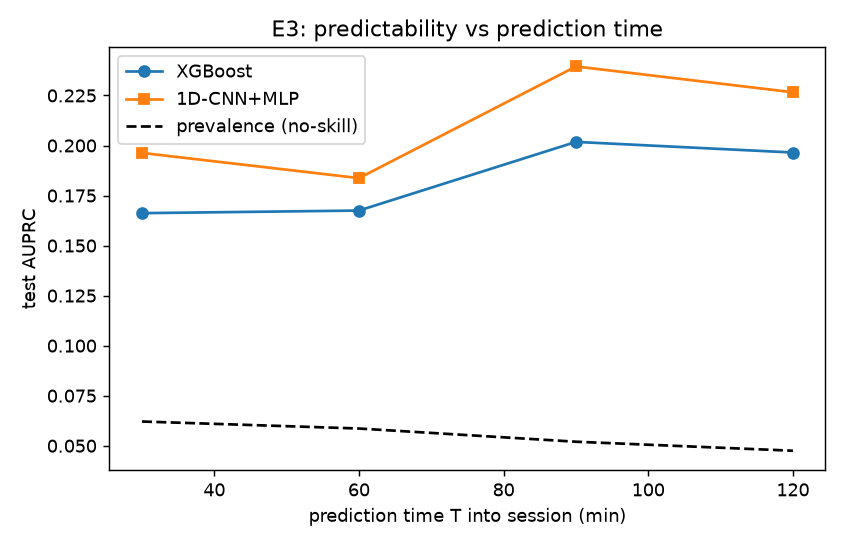
\includegraphics[width=0.49\linewidth]{figs/fig_e3_horizon.png}
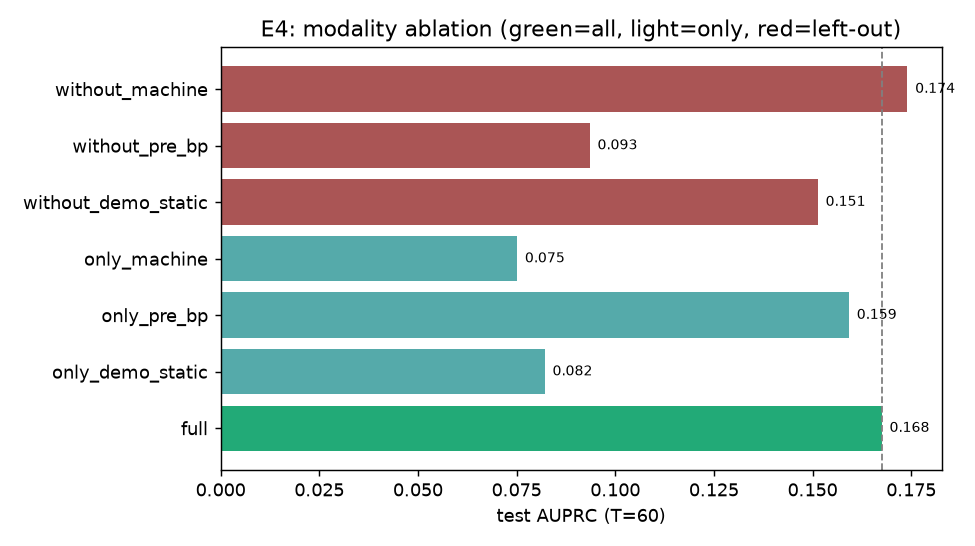
\includegraphics[width=0.49\linewidth]{figs/fig_e4_ablation.png}
\caption{Left: E3 horizon curve against the prevalence (no-skill) line. Right: E4 modality ablation.}
\label{fig:e3e4}
\end{figure}

\paragraph{E4: modality ablation.} Table~\ref{tab:e4} answers the sensor question. Pre-$T$ blood-pressure history alone nearly matches the full feature set (0.1592 versus 0.1675), and removing it costs 44\% of AUPRC --- the largest single loss. Machine settings alone are weak (0.0751), and removing them slightly \emph{improves} the model (0.1740), indicating little independent signal at $T$=60; this is consistent with clinicians already reacting to blood pressure, so the UF setting partly encodes that reaction. Static demographics contribute a small but non-zero amount. Within this data, then, physiological sensing carries the signal and additional machine-side channels do not. We stop short
of the stronger claim that adding a high-frequency sensor such as photoplethysmography would improve prediction: the current
data contain no such signal, so that remains a hypothesis for the next study rather than a result here. Caveat: this ablation
uses XGBoost; sequence models might extract more from the dense machine stream, which we leave as follow-up.

\begin{table}[t]
\caption{E4: modality ablation (XGBoost AUPRC, $T$=60). ``Only'' uses one group; ``w/o'' drops one group.}
\label{tab:e4}
\centering
\begin{tabular}{lc}
\toprule
Feature set & AUPRC \\
\midrule
All 15 features & 0.1675 \\
Only pre-$T$ physiology & 0.1592 \\
Only demographics/static & 0.0821 \\
Only machine settings & 0.0751 \\
Without pre-$T$ physiology & 0.0935 \\
Without demographics/static & 0.1513 \\
Without machine settings & 0.1740 \\
\bottomrule
\end{tabular}
\end{table}

\paragraph{E5: exploratory action-conditioned risk simulation.} This section is a sensitivity analysis, not a test of a
control policy, and we label it accordingly. Two earlier versions were withdrawn: the first anchored candidates on the UFR
actually delivered \emph{after} $T$, which is unavailable at decision time; the second anchored them on the mean rate
delivered so far, which is not the rate the machine is running. The current anchor is the \textbf{pump setting observed at
$T$} (the last non-zero setting at or before $T$; mean 0.70 against 0.62 for the historical mean, correlation 0.80), with
candidates $\{1.0,0.9,0.8,0.7,0.6\}\times$ that setting. Arms are \emph{hold}, \emph{reactive} (cut 30\% if SBP has fallen
$\ge$15~mmHg or nadir is below 100), and \emph{predictive} (minimise predicted risk subject to a residual-fluid tolerance).
The plan clinicians followed is a descriptive reference only. Risks are Platt-recalibrated, fitted on validation.

Table~\ref{tab:e5} reports the arms at $T$=60~min with patient-level bootstrap intervals. The ordering is
hold (7.3\%) $>$ reactive (7.2\%) $>$ predictive (5.9\%), and it costs fluid to move down that ordering: 131~mL residual for
hold, 239~mL for reactive, 354~mL for predictive. Marginal intervals overlap, which on its own would be the wrong test; paired patient-level bootstraps
on the risk \emph{differences} put hold above predictive by 1.41 points (95\% CI 1.12--1.74) and reactive above predictive by
1.30 (1.06--1.60), while hold and reactive are indistinguishable (0.11, $-0.06$ to 0.25). So the model does order the arms;
what it cannot do is establish that the ordering would survive in patients, because the same model both chose and scored the
action, and because 65\% conditional support leaves a third of the candidates outside comparable practice.

Three further limits. (i) \emph{Conditional} overlap is weaker than marginal overlap: 88\% of candidates lie inside the
overall observed range of post-$T$ plans, but only 65\% lie inside the 10--90 percentile of plans used for patients in the
same pre-$T$ nadir and interdialytic-gain stratum. That is a stratification on two pre-decision covariates, not a
demonstration of causal overlap: most of the apparent marginal support is between-patient heterogeneity. (ii) The
same model both selects and scores the action, which biases the selected arm optimistically; a second, independently seeded
model (depth 3, no class weight) reproduces the ordering but shifts every level up by 0.6--1.3 points, with per-sample
correlations of 0.85--0.87. (iii) Calibration is established on the factual distribution; it says nothing about calibration
under counterfactual treatment, so the calibrated numbers remain conditional-risk estimates.

\begin{table}[t]
\caption{E5: exploratory action-conditioned risk simulation at $T$=60~min (tolerance 0.5~L). Intervals are
patient-level bootstrap ($B$=500). Arms are model outputs under a conditional-risk model. Marginal intervals overlap, but paired patient-level
differences do exclude zero (see text); neither establishes a treatment effect.}
\label{tab:e5}
\centering
\begin{tabular}{lccc}
\toprule
Arm & Predicted risk (95\% CI) & Residual fluid (95\% CI) & Extra time \\
\midrule
Observed plan (reference) & 5.8\% (4.9--7.0) & 699~mL (599--830) & 120~min \\
Hold setting at $T$ & 7.3\% (6.2--8.6) & 131~mL (89--190) & 13~min \\
Reactive rule & 7.2\% (6.1--8.5) & 239~mL (184--312) & 28~min \\
Predictive & 5.9\% (5.0--7.0) & 354~mL (288--453) & 50~min \\
\bottomrule
\end{tabular}
\end{table}

\begin{figure}[t]
\centering
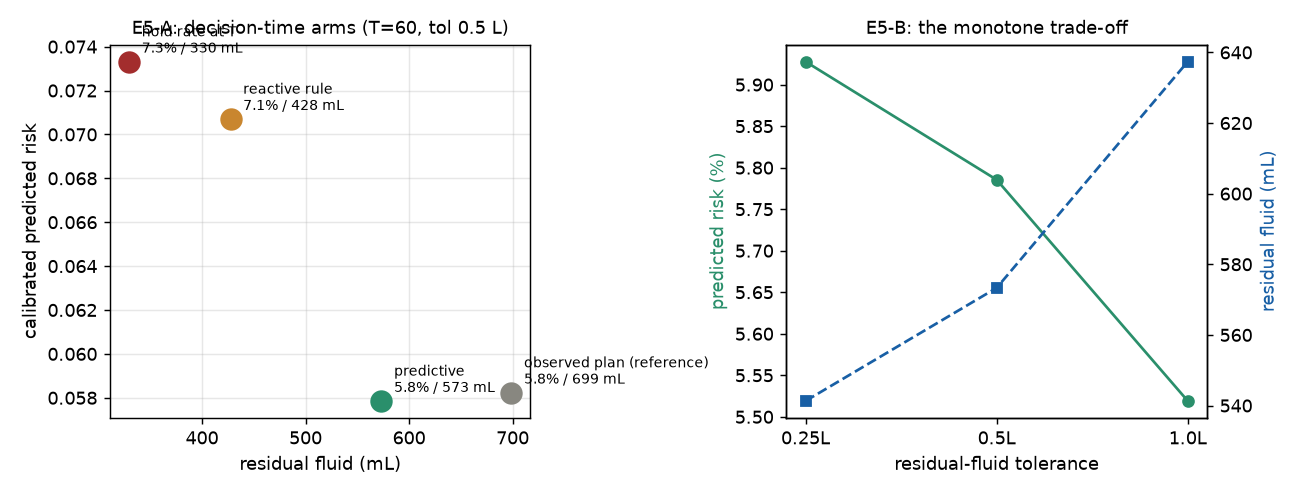
\includegraphics[width=0.95\linewidth]{figs/fig_e5_tradeoff.png}
\caption{E5: the IDH-versus-fluid trade-off (left) and its sensitivity to the residual-fluid tolerance (right).}
\label{fig:e5}
\end{figure}

\paragraph{E6: causal plausibility diagnostics.} Figure~\ref{fig:e6} reports both probes. The perturbation sweep is monotone and in the expected direction: raising the planned remaining UFR multiplier from 0.3 to 1.3 raises mean predicted risk from 0.183 to 0.265 (gradient $+0.089$). The crude association agrees: binned by actual post-decision UFR, observed IDH rises from 3.1\% to 11.8\%. This is necessary for the control simulation to make sense --- but it is not sufficient to establish causality, because confounding by indication predicts the same pattern: patients who are more fluid-overloaded, and therefore more fragile, receive higher ultrafiltration and are also more likely to become hypotensive. The monotone response is an internal consistency check for the model-based simulation --- it shows the model reacts to UFR
in the expected direction --- but it does not validate predictions for actions that were not taken, nor does it establish a
causal effect; its magnitude cannot be decomposed into causal and confounded parts from this data.

A second probe is more surprising. Zeroing the attention output of each Transformer encoder block changes the logit by about $10^{-8}$ --- effectively nothing --- whereas zeroing the feed-forward output changes it by 0.042 and 0.067 at layers 0 and 1. The predictive signal therefore flows through the feed-forward path, not through attention, over a sequence of roughly 22 readings with sparse blood pressure. Two consequences follow: attention-heavy architectures are hard to justify here (reinforcing E1/E2), and attention maps must not be presented as clinical explanations --- the same observation-versus-intervention lesson from our earlier coursework.

\begin{figure}[t]
\centering
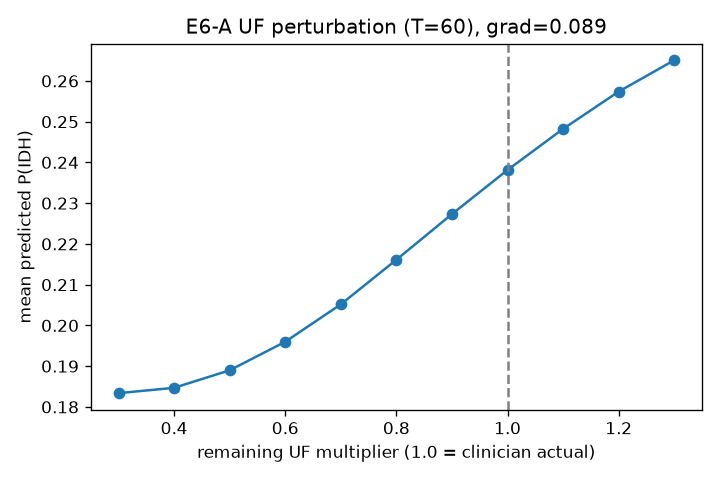
\includegraphics[width=0.49\linewidth]{figs/fig_e6_perturb.png}
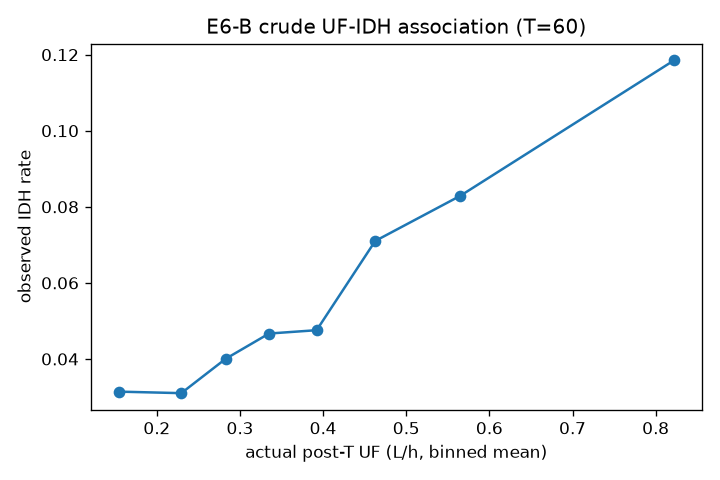
\includegraphics[width=0.49\linewidth]{figs/fig_e6_empirical.png}
\caption{E6: left, predicted risk under UFR perturbation; right, crude observed UFR--IDH association. Both are consistent with a causal effect and with confounding.}
\label{fig:e6}
\end{figure}

\paragraph{E7: hyperparameter sensitivity.} Hyperparameters are selected on the validation split; the test split is
reported only for the selected configuration. For XGBoost, tree depth dominates validation AUPRC: depth 3 reaches 0.32 and
depth 9 falls to 0.18, with 200 trees preferred over 600 or 1200 (Figure~\ref{fig:e7}). The validation-selected configuration
(n=200, depth 3) scores 0.186 on test, against 0.168 for the default (n=600, depth 6). For the 1D-CNN+MLP, the learning rate
matters more than the class weight: $3\times10^{-4}$ is best on validation and gives 0.194 on test, against 0.188 at $10^{-3}$.

One caveat matters more than the numbers. Validation and test disagree about the \emph{ranking} of these configurations ---
the configuration with the best test score (n=600, depth 3, 0.190) ranks below the best validation score (n=200, depth 3) ---
which is the same instability that inflates validation AUPRC in E1. At this sample size, hyperparameter selection is not
stable enough to support a claim that tuning improves the model; we therefore report E7 as a sensitivity analysis rather than
a tuning result, and E1 keeps identical defaults across models so that the comparison holds the pipeline constant.

\begin{figure}[t]
\centering
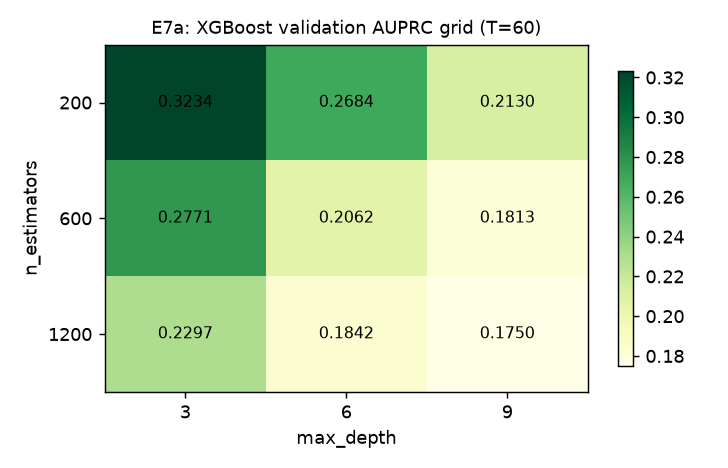
\includegraphics[width=0.49\linewidth]{figs/fig_e7_xgb_grid.png}
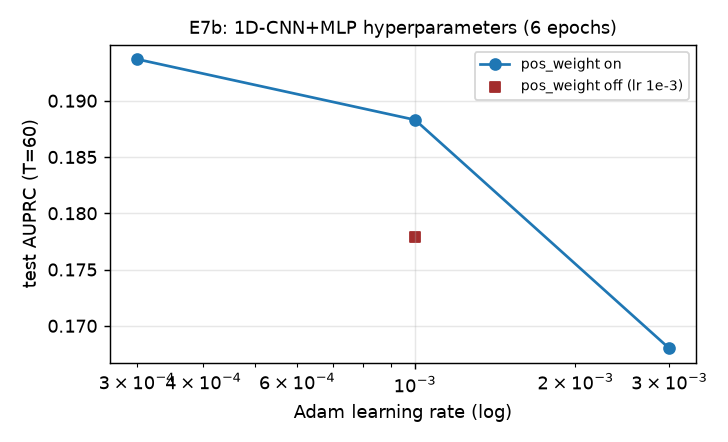
\includegraphics[width=0.49\linewidth]{figs/fig_e7_nn_lr.png}
\caption{E7: hyperparameter sensitivity. Left: XGBoost validation AUPRC over tree depth and ensemble size (selection split).
Right: 1D-CNN+MLP learning-rate sweep with and without positive-class weighting.}
\label{fig:e7}
\end{figure}

\paragraph{E8: are the probabilities usable as risks?} No, not before recalibration. Table~\ref{tab:e1} already shows that
every Brier score exceeds the no-skill value $p(1-p)=0.0552$, and Figure~\ref{fig:e8} shows why: mean predicted probabilities
are 0.24--0.35 against an observed 0.0586, an over-prediction of four to six times, with calibration slopes of 0.56--0.82
rather than 1. The cause is the training recipe, not the architecture: \texttt{scale\_pos\_weight} (and
\texttt{pos\_weight}) reweights the loss by 17:1, which shifts the effective prior, and no step maps the resulting scores
back onto the observed event rate. Fitting standard two-parameter Platt scaling --- a slope and an intercept on the logit, both estimated on the validation
split --- and evaluating it \emph{on the untouched test split} repairs the probabilities without touching the ranking: Brier falls to 0.0515--0.0525 for all five models, below the
no-skill 0.0552, while AUPRC is unchanged by construction. The improvement is real but modest --- a Brier skill score of only
4.9--6.7\% relative to the no-skill forecast --- so the correct reading is that the probabilities carry some information, not
that they are accurate enough to drive a clinical decision. Nor does calibration transfer to counterfactual actions: the map
is fitted on the distribution of treatments clinicians chose, so nothing here licenses calibrated risk under a treatment that
was rarely or never given. Two consequences follow. First, ``best Brier among five'' in E1 does not
mean well calibrated --- it means least bad before repair. Second, every risk level quoted in E5 is recalibrated; raw scores
would have overstated risk by roughly a factor of four, and a control policy optimising raw scores would be optimising a
distorted objective.

\begin{figure}[t]
\centering
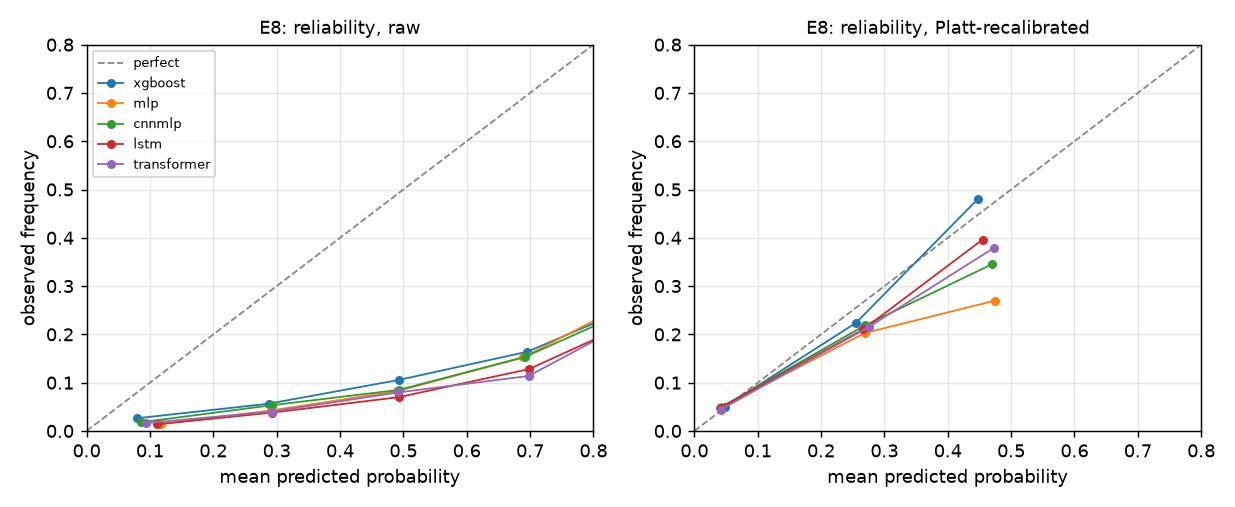
\includegraphics[width=0.92\linewidth]{figs/fig_e8_reliability.png}
\caption{E8: reliability diagrams before (left) and after (right) Platt recalibration. Raw predictions fall below the diagonal,
which denotes overprediction; two-parameter Platt scaling improves their alignment with the diagonal on the held-out test set,
though it does not make them coincide. Because the raw slopes were 0.56--0.82 rather than 1, the slope term is doing real work:
an intercept-only correction would not have fixed the compression.}
\label{fig:e8}
\end{figure}

\paragraph{E9: is the model ordering real?} No. Bootstrap resampling by patient ($B$=1{,}000) gives 95\% intervals of
0.118--0.221 (XGBoost), 0.117--0.268 (1D-CNN+MLP) and 0.131--0.282 (Transformer); the paired difference between the
Transformer and the fusion model is 0.018 with an interval of $-0.001$ to 0.033, positive in 96.6\% of resamples. A 96.6\%
one-sided figure is suggestive but the interval crosses zero, and after the hyperparameter sweep in E7 the gap narrows to
0.009. We therefore report the comparison as ``competitive at a quarter of the parameters'' rather than ``better''. Any
product decision that hinges on the ranking would need either far more patients or an external cohort.

\paragraph{Software 3.0 in the experimental workflow.} Two of the seven experiments exist because of an AI-assisted check rather than a planned one: the probability-versus-logit diagnosis that produced the whole-test-set sanity check, and the suggestion to test attention against feed-forward ablation once the attention heatmaps looked uniform. In the other direction, the first session builder proposed for this project died on 160k sessions; the vectorised rewrite was suggested, but confirming that no patient crossed a split still had to be done by hand. The recurring pattern was that assistance shortened the distance from a symptom to a candidate cause, and contributed nothing to deciding which claim the evidence licenses.

\section{Discussion and Conclusion}

\paragraph{What we can now say.} Three questions were asked at the outset. First, how early and how accurately: with routine machine data and sparse cuff pressures, IDH is predictable at a
60-minute horizon with AUPRC 0.2015 against 0.0586 prevalence (AUROC 0.774) --- but with an interval of 0.13--0.28, and no
established advantage over a compact fused model at a quarter of the parameters. Second, whether multi-modal sensing is necessary: only intra-session blood pressure is indispensable; machine settings contribute almost no independent signal at $T$=60. Third, what prediction buys and costs: within the simulation, moving from holding the observed rate to a model-chosen
reduction lowers predicted risk from 7.3\% to 5.9\% while leaving 223~mL more fluid behind, and the intervals overlap --- the model produces a consistent predicted-risk--fluid trade-off within this
simulation, but neither its direction nor its magnitude is identified as a treatment effect, because the model is
conditional rather than counterfactual.

\paragraph{What the operating point would mean clinically.} AUPRC does not by itself establish clinical value. At 80\%
specificity the Transformer reaches 0.587 sensitivity; at the test prevalence of 5.86\% this implies a positive predictive
value of about 15\%, i.e.\ roughly 3.4 true events and 18.8 false alarms per 100 sessions. Whether that is usable depends on
what an alarm triggers --- a nurse review, a patient prompt, an automatic reduction --- and on the relative cost of a missed
hypotensive episode versus a repeated false alarm. Neither cost is observable in this dataset: there are no symptom records,
no intervention logs and no workflow data. The threshold, the alarm burden per session or per hour, and the action that
follows therefore remain design decisions to be settled in a prospective study, not quantities this analysis can supply.

\paragraph{Boundaries we will not overstep.} Every control number here is in silico under a model trained on clinicians' own decisions; it is not clinical validation. The dose--response gradient is equally compatible with confounding by indication, so the simulated differences are neither
estimates nor bounds of a treatment effect: the direction and magnitude of any real clinical benefit remain unidentified in
these observational data. The attention-ablation result means explanation should not be read off attention weights. And the cohort is in-centre haemodialysis with a cuff measurement every 50.7 minutes: it cannot speak to the ambulatory wearable scenario, which lacks exactly the high-frequency modalities
(photoplethysmography, inertial, pressure waveforms) whose value this dataset cannot measure --- the ablation says blood
pressure history matters, not that a new sensor would help. Scaling from 4-hour supine sessions to 6--8-hour ambulatory therapy, and from sparse to continuous sensing, remains an extrapolation that this dataset cannot adjudicate.

\paragraph{Implications for the design project.} The results strengthen three claims and weaken one. Strengthened: physiological information is where the predictive signal sits within this dataset, which supports studying how
it should be captured rather than settling a sensor budget (E4) --- the incremental gain, cost and practicality of continuous
monitoring or photoplethysmography need their own data and experiment; a compact convolutional-plus-MLP model is a credible
deployment shape, since it is competitive under the default comparison while being far cheaper (E1/E2); and a clinician-set
safety envelope with a hard physical override is not bureaucratic decoration but a necessary condition, precisely because the
causal strength of ultrafiltration cannot be established retrospectively (E6). Weakened: the design project's framing of its contribution as ``prediction beats PID'' is historically inaccurate --- 28 clinical studies of closed-loop ultrafiltration biofeedback predate it \citep{dong2024closedloop}. The more defensible framing is narrower: \emph{testing whether routine machine data and inference can reduce reliance on an
optical relative-blood-volume sensor}. This study provides grounds to research that question; it does not show that routine
data can replace the sensor, nor that adding photoplethysmography would improve prediction. The five-to-fifteen-minute warning specification also needs restating, since it is not verifiable on routine data and depends on the continuous sensing the device is meant to provide.

\paragraph{What the project taught me.} The value of a healthcare-AI contribution sits less in the highest AUPRC than in knowing which claim the data can carry. The most useful result here is a negative one --- that the control policy cannot be validated retrospectively --- and it took a controlled model comparison, a modality ablation and an intervention probe to establish it rather than assert it.

\paragraph{Future work.} Four directions follow directly. External validation on a second centre, since all results here come from one cohort. A properly validated calibration step deployed with the model: Platt scaling works but was fitted on a single split, so it needs external confirmation before any threshold is used clinically. A targeted-causal analysis --- within-patient comparisons or instrumental variables --- to bound the causal share of the ultrafiltration gradient. And a high-frequency simulation arm, calibrated to the distributions reported here, to test whether the ambulatory scenario preserves or reverses the conclusions.

\paragraph{Conclusion.} What this study delivers is narrower than a closed-loop device: an offline risk-prediction pipeline
and an exploratory action-conditioned sensitivity analysis, both reproducible on routine data, plus a quantified account of
the predicted-risk--fluid trade-off and of why the data cannot settle the causal question. Sensor-light closed-loop control
remains a hypothesis for development --- one with a clear evidence ladder (external validation, alarm burden, target-device
observation, clinician-in-the-loop decisions, and only then automated control), not a demonstrated capability.

\bibliographystyle{plainnat}
\bibliography{references}

\end{document}
